%!TEX root = report.tex
\chapter{Background}

\section{London Bus Network}

\par The bus network in London is one of the largest and most accessible in the world. It carried a staggering number of passengers with more than 2.4 billion journeys in 2013/14, which was more than any year since 1959 \cite{tfl_annual_report_13/14}.
On an average day during 2005 -- 2010, London residents made 14\% of their trips by bus \cite{tfl_ltds}, pending an average of 14 minutes per day on the bus.
As at 2015, there are 19,345 bus stops with 680 routes served by 8,765 buses daily in London \cite{bus_stop_locations_routes}.

% \todo[inline, color=purple]{produce graph for this, number of stops, routes and buses}
% number of people that use apps to plan journey or pick the bus to take

\subsection{Bus Network Performance}

\par Bus service delays and disruptions are commonplace in London. Such delays can significantly affect the estimated duration of a route.

\par \textbf{High frequency services.} The average scheduled wait was 4.86 minutes, the average excess wait was 0.94 minutes, and the average actual wait was 5.80 minutes. While passengers could expect  buses to arrive within 10 minutes 83.4\% of the time, there was a 15.1\% chance of a 10-20 minute wait, a 1.3\% chance of a 20-30 minute wait, and a 0.2\% chance of a wait exceeding 30 minutes.

\par \textbf{Low frequency services.} 87\% of buses services were on time, and 11.4\% were 5-15 minutes late.

\par \textbf{Night buses.} 84.5\% of services were on time. The average excess wait was 0.68 minutes.

% \todo[inline, color=purple]{produce graph here}

\par Causes of bus delays included traffic congestion, staff availability, engineering problems, or mechanical breakdown \cite{buses_performance_data}. The above statistics were published in TfL's 2014/2015 Q2 bus performance data \cite{buses_performance_report}.


\section{Buses Status Updates}

\par The frequency of bus delays makes it essential for an estimate of the length of a bus journey to incorporate estimated delays based on live bus tracking data.
To inform passengers of bus service disruptions or diversions, \acrshort{tfl} provides a bus status updates service online \cite{tfl_buses_status_updates}. Passengers can check the service status of a given bus stop or route (Figure \ref{fig:tfl_status_update}).
The status update consists of textual descriptions of service disruptions, diversion, suspensions, and delays due to heavy traffic.
While this service allows passengers to discover disruptions on their route, it requires passengers to actively monitor the site, and does not quantify the effect of the disruptions in extending the passenger's travel time.

\begin{figure}
\centering
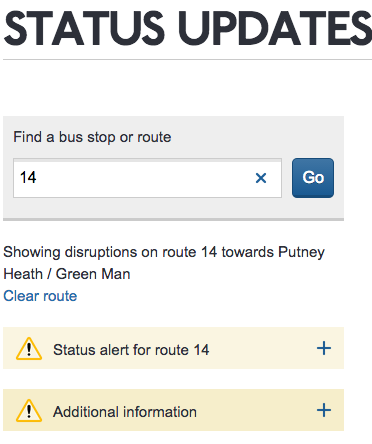
\includegraphics[width=0.5\textwidth]{figures/tfl_status_update.png}
\caption{\label{fig:tfl_status_update} Tfl Buses Status Update Service}
\end{figure}

\par \acrshort{tfl} also publishes live status news and updates on Twitter \cite{tfl_bus_alerts_twitter}. This has the advantage of making the information more easily accessible to passengers. However, the general broadcast does not solve the problem of giving passengers information that is specific to their planned journey.

\par Many popular journey planners such as Google Maps \cite{google_maps}, Citymapper London \cite{citymapper}, and \acrshort{tfl} Journey Planner incorporate the bus status information in the suggested journeys as a textual alert. However, these applications do not calculate the additional time that the service disruption will add to the journey, leaving passengers to estimate this for themselves.

\par Thus, it can be clearly seen that no solution currently exists which is able to quantify the additional delay that a disruption adds to a journey, and incorporate those predicted delays into time estimates of different routes presented to a commuter.

% \section{Choice of Travel Mode}
% \todo[inline]{Does the arrival time / delay affect people's choice of travel mode? What are the purposes of commute? Work, travel, leisure, appointments?}
